%%%%%%%%%%%%%%%%%%%%%%%%%%%%%%%%%%%%%%%%%%%%
%%% GRIMOIRE TRAPS
%%%%%%%%%%%%%%%%%%%%%%%%%%%%%%%%%%%%%%%%%%%%

\end{multicols*}
\mysection{Grimoires and Fetishes}{inscription-grimoires-fetishes}



\mysubsection{Grimoires}{grimoires}

Grimoires are solid, heavy books with thick pages and sturdy covers, containing the definitive copies of the Secrets you know. This makes them cumbersome and difficult to read - in Combat, finding the right page and speaking the Secret requires \mybold{2 Maneuver Actions} (this doesn't include the time it takes to fish it out of your pack!).

Runes and symbols confine the \mylink{Secrets}{arcana-wizardry-secrets} inside the Grimoire in cages of crystallized thought. Each tome contains enough room for 10 Secrets. Some Secrets must be stored across several pages for safety, so the books contain more than 10 pages, and have plenty of room for notes, ledgers, or sketches - and curses, hexes, coded and cryptic entries written with poisonous and hallucinogenic inks (see below). Grimoires come in a waterproof, acid- and fire-resistant bag. Outside the bag, they are not waterproof and are quite flammable. You can buy a blank (and unbound) Grimoire in a \mylink{Settlement}{gear-equipment}.

When you purchase a blank \mylink{Grimoire}{gear-equipment}, you must first place a \mylink{Wizard Sigil}{inscription-sigil-wizard} on the frontispiece before you begin placing Secrets inside of it. If your Wizard Sigil is ever erased, the Grimoire folds in on itself and disappears (permanently) into the Void, taking its Secrets with it.

The contents of any Grimoire are a web of shorthand, calligraphy, sketches, marginalia, footnotes, and cross-references only understood by you, barely keeping the Void confined within. Anyone who reads the contents of a Grimoire before they are \mylink{Translated}{inscription-translation} must immediately roll on the \mylink{Grimoire Traps}{grimoire-traps} table and suffer the fate outlined therein. 


\mysubsection{Fetishes}{fetishes}

Fetishes are ways of making Secrets portable and easy to use in Combat. A Fetish can be a papyrus, set of mouse skulls, handle of an axe, roll of snakeskin, etc. but cannot be inscribed on anything alive.  A Fetish can only contain a single Secret; in Combat, speaking a Secret inscribed on a Fetish requires \mybold{1 Maneuver Action} (this doesn't include the time it takes to fish it out of your pack, if applicable).

Fetishes are "magical" in and of themselves, but lose their potency after repeated use. All Fetishes have a \UDD{d4} - when the \UD is exhausted, the magical words disappear from the Fetish. 

See the section on \mylink{Inscription}{research-inscription} for details on how to create Fetishes.

\begin{center}
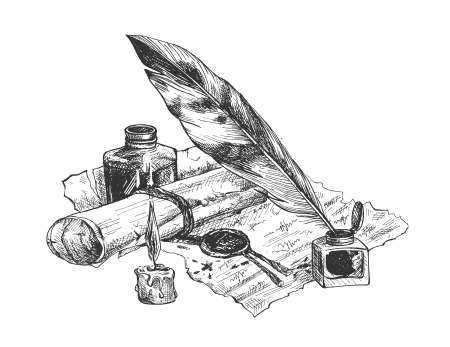
\includegraphics[scale=.4]{research/Ink}
\end{center}
\newpage

\mysubsection{Grimoire Traps}{grimoire-traps}

\ed{Once again, thanks be to Logan Knight for \href{https://www.lastgaspgrimoire.com/cunning-linguists/}{Cunning Linguists?}}


  \mytable{l X} {  
  } {
        1 &  The Grimoire bursts into flame like a pile of magnesium, destroying it. \\
        2 &  Tiny hideous mouths split open over the surface of the Grimoire and begin to scream and never stop. \\
        3 &  Heat emanates from the page and you absent-mindedly place your hand against it to feel the warmth. The ink burns into your skin like a tattoo. A lie you tell will become true (Arbiter's discretion), and the writing on your hand will change to remind you of that for all time. \\
        4 &  The Grimoire cover grows course and hairy, legs sprout from the spine and it leaps from your hands, running across the room and up the wall. It points a strange cloaca at you from the base of its spine and expels clumps of bright green mildew at you that burns the skin, flapping away to the other side of the room if you get too close. \\
        5 &  The edges of the Grimoire slice your fingers open before it drops to the floor, leaving tiny rows of perfect bloodless papercuts. They will never heal, and from this moment forth you will bleed prose. It is not for me to know what secrets may be found in your blood. \\
        6 &  Cold pink mist swells up from the Grimoire and wafts out; everyone Close or Nearby must \SAVE{Doom} or lie down to sleep in a blanket of fog for Years (unless slapped awake). \\
        7 &  The words seem to drive themselves through your pupils, expanding from within and showering your companions with optic fluid. In place of your eyes remain two rolling black orbs, words and phrases wafting from them like smoke. Somehow you remain able to see, and much hidden knowledge can be learned by anyone studying your eyes (+4 to Skill: Lore tries). However, if you spend time looking at your own reflection you must make an \INSANITY try every Minute.  \\
        8 &  Violet light flashes from the pages, and in your temporary blindness you can hear the resonance of your own thoughts. When you look back at the book you are staring at your own placid face, when you cry out it is the face in the book that opens its mouth and screams, not the featureless mess of words plastered around your swollen eyes. \\
        9 &  You birth a wriggling pink rat with a young version of your own face out of your mouth. It scrambles away and out of sight. It will grow to about the size of a pug, it develops translucent flaps of skin to glide on, it keeps showing up to foil your plans. \\
        10 &  Tendrils snap out from the crease of the Grimoire, penetrating your chest and belly, churning as some drain and others pump. Your organs liquefy and drain out with your blood, and in its place your body fills with fluid like liquid golden light. You glow like a pinkish-gold beacon, and take a -4 penalty to your Save vs. Doom, but you are immune to Toxins and gain 1 Blood Die. \\
        11 &  After you shut the Grimoire, the cover creaks back open and oily dripping creatures begin to pull themselves from a portal within. Their form is myriad and shifting, they merge and split and far-off tittering fills the air. To close the portal you have only to shut the Grimoire again, but the floor is crawling with flesh like oil. \\
        12 &  The pages of the Grimoire begin to flip back, growing faster, pulling at the air around you, the flurry of paper flipping between the covers of the book consists of more pages than the book could possibly have contained. The pull at the air around you grows stronger, small objects begin to lift from the floor and disappear between  the pages, your feet begin to shift... \\
  }

\newpage

  \mytable{l X} {  
  } {
    13 &  Vines emerge from the cover of the Grimoire, growing lush and dense as leaves and fleshy flowers sprout from them. There are enough vines to fill a 10m cubed room, and the flowers bloom to reveal a glistening red interior filled with shivering barbs. Anyone shot by the barbs is immediately \mylink{Befuddled}{effect-befuddled} for \DUR{d20} unless they \SAVE{Doom}. \\
    14 &  Bronze threads burst from the walls, roof, even the Grimoire, and sew into your flesh. If you move more than a few inches parts of your body start to tear away. You being \mylink{Bleeding}{effect-bleeding}. Someone will need to cut you free. \\
    15 &  Fragrant mud pools within the letters and begins to spill down the Grimoire and crabs with voices like angels emerge from the pooled muck and beseech to be allowed within you. They're actually quite persuading - \SAVE{Doom} or allow the angelcrabs inside your mouth, and eyes, and various other orifices. They eat their fill and excrete muddy gold in their wake to excavate a home, causing d12 damage directly to Flesh. If you survive the experience the angelcrabs will live in symbiotic harmony within your body, imparting alien wisdom when they deem it appropriate (+4 to Skill: Lore tries, among other "benefits" at the Arbiter's discretion). \\
    16 &  The words on the page begin to quiver, the ink contracts and swells and forms drops of dark rain which fall up from the Grimoire. Soon the paper itself is raining away, while the Grimoire's cover becomes ever more heavy in your hands. After the rain the inner cover clears to reveal a glimmering night sky, full of constellations you've never known. They swirl and dance and you step into the vastness of their glory, held by their cosmic light in an eternity of tormenting discovery. The rain falls back down in a torrent, replacing pages and letters and phrases until the Grimoire slams shut. If the Grimoire is opened you will return, but you will not return the same as you once were. Make an \INSANITY try - if you roll a Failure, roll 3 times on the \mylink{Madness!}{injury-insanity-madness} table (in lieu of the normal results for \INSANITY).  Additionally, you must \SAVE{Doom}; if you fail, roll 3 times on the \mylink{Night Child}{species-night-child} Complications table and apply the results to yourself. Regardless of your rolls, you do not return alone, the star spawn's seed rests in your belly and in your mind, waiting. \\
    17 &  Beads of amber sweat, swell, and glisten over the Grimoire's surface; it begins to look more pliant, more organic, its bulk starts to heave in labored breaths.  Sections split away in mockery of limbs, pools of flesh swirl inwards forming gaping circular mouths, their inner surface full of quivering jelly-like teeth. The hunt begins. \\
    18 &  Shadows thicken behind you, whispering as they gain density, reaching out, grasping at your heels. The room swells with viscous shadow, breathing limbs reach into your body and twist your veins, the door is shut and covered in a thick layer of quiet loathing.  You no longer need food or drink or sleep, and you cannot leave this room. \\
    19 &  Bright light blasts from the open Grimoire and melts your face, a la \myital{Raiders of the Lost Ark}. \SAVE{Doom} or die. If you succeed, your head is now a naked skull, covered in weird crawling runes. \\
    20 &  The words snake off of the page and across your skin, circling around your limbs and across your chest until your entire body bears the contents of the Grimoire. You fall to the floor in agony as the tiny circlets of writing brand into your flesh. The deathless librarians of the \mylink{Stygian Library}{atlas-stygian-library} cannot help but seek and catalog the Living Word, and they always know when a new one has been created. 
  }

\begin{multicols*}{2}
